\section{Large-Width Regime: Comparison with Prior Result}\label{sec:exact}
In the `large-width' regime, as $w\ra\infty$, in \eqref{eq:graddyna}we have $\dot{\Theta}_t, \dot{\phi}_t, \dot{v}_t\ra 0$, and the error dynamics is given by
\begin{align}
\dot{e}_t=-K^{(d)} e_t,
\end{align}
since, as $w\ra\infty$, $K_{\Theta}$ in \eqref{eq:graddyna} converges to $K^{(d)}$ in \eqref{eq:ntkold} with $\chi=\chi_{sr}$. 
\begin{align}\label{eq:ntkold}
&\tilde{K}^{(1)}(s,s')=\Sigma^{(1)}(s,s')=\Sigma(s,s'), M^{(l)}_{ss'}=\left[\begin{matrix}\Sigma^{(l)}(s,s) & \Sigma^{(l)}(s,s')\\ \Sigma^{(l)}(s',s) & \Sigma^{(l)}(s',s')\end{matrix}\right]\in \R^2,\\
&\Sigma^{(l+1)}(s,s')= 2\cdot\mathbb{E}_{(q,q')\sim N(0,M_{ss'}^{(l)})} \left[\chi(q)\chi(q')\right], \dot{\Sigma}^{(l+1)}(s,s')= 2\cdot\mathbb{E}_{(q,q')\sim N(0,M_{ss'}^{(l)})}\left[\dot{\chi}(q)\dot{\chi}(q')\right],\nn\\
&\tilde{K}^{(l+1)}=\tilde{K}^{(l)}\odot \dot{\Sigma}^{(l+1)}+\Sigma^{(l+1)},\nn
\end{align}
where $s,s'\in[n]$ are two input examples in the dataset, $\Sigma$ is the data Gram matrix, $\dot{\chi}$ stands for the derivative of the activation function with respect to the pre-activation input, $N(0,M)$ stands for the mean-zero Gaussian distribution with co-variance matrix $M$. The final limiting matrix is given by $K^{(d)}=\left(\tilde{K}^{(d)}+\Sigma^{(d)}\right)/2$. 

In prior works, in the expression for the limit NTK $K^{(d)}$ in \eqref{eq:ntkold}, $\chi$ was either $\chi_r$ (the standard ReLU) or $\chi_{sp}$ (known as the soft-plus), wherein, $\dot{\chi}_r$ is a Heaviside step function and $\chi_{sp}$ is a logit function. Both these functions capture only the \emph{on/off} behaviour of the gates, and hence $K^{(d)}$ captures only the flow of value gradient. On the contrary, in the case of soft-ReLU, $\dot{\chi}_{sr}$ contains both the \emph{on/off} information via the $\dot{\chi}_{sp}$ term as well as the information on the dynamics of sensitive gates via the $\dot{G}_{sr}$ term. Plugging the soft-ReLU instead of softplus/ReLU in \eqref{eq:ntkold} will indeed bring in the additional as below:
\begin{align*}
\dot{\Sigma}^{(l+1)}(s,s')&=\dot{\Sigma}^{(l+1)}_v(s,s')+ \dot{\Sigma}^{(l+1)}_{\phi}(s,s') + \dot{\Sigma}^{(l+1)}_{cross}(s,s'),\text{where}\\
\dot{\Sigma}^{(l+1)}_v(s,s')&=2\cdot\mathbb{E}_{(q,q')\sim N(0,M_{ss'}^{(l)})}\left[\dot{\chi}_{sp}(q)\dot{\chi}_{sp}(q')\right],\\
\dot{\Sigma}^{(l+1)}_{\phi}(s,s')&=2\cdot\mathbb{E}_{(q,q')\sim N(0,M_{ss'}^{(l)})}\left[\dot{G}_{sr}(q)\dot{G}_{sr}(q')\right]
\end{align*}
However, in the `large-width' regime, $\dot{\theta},\dot{\phi},\dot{v},\dot{K}\ra 0$, and hence distinctions between $K^{v}_{\Theta}, K^{\phi}_{\Theta}$ does not make much difference. In this regime, only the fixed $K^{(d)}$ matters.
\begin{comment}
\subsection{Explicit Gate Dynamics: soft-ReLU vs softplus}
\FloatBarrier
\begin{figure*}[h]\centering
%\begin{minipage}{0.78\columnwidth}
\resizebox{\columnwidth}{!}{
\begin{tabular}{ccc}
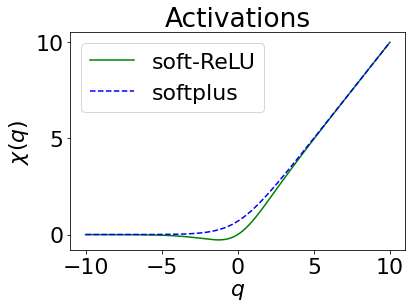
\includegraphics[scale=0.4]{figs/act.png}
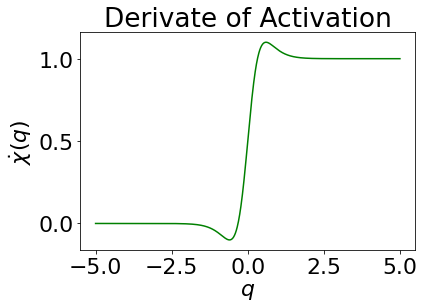
\includegraphics[scale=0.4]{figs/der-act.png}
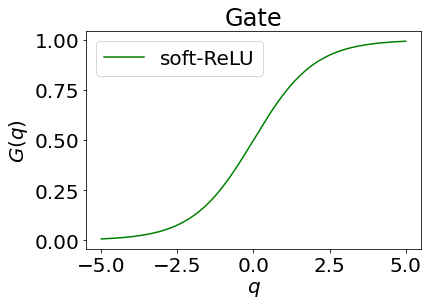
\includegraphics[scale=0.4]{figs/gate.png}
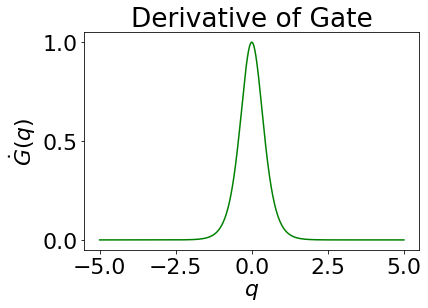
\includegraphics[scale=0.4]{figs/der-gate.png}
%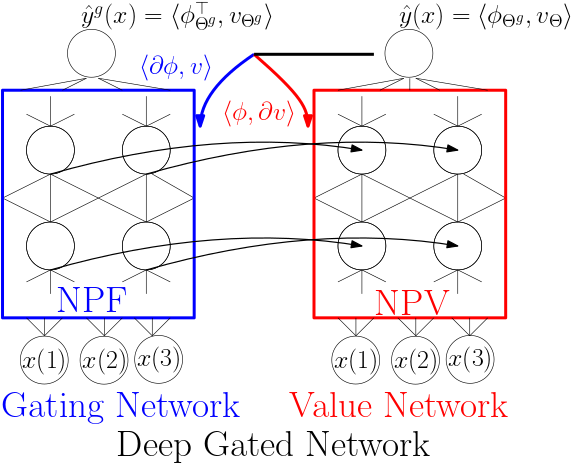
\includegraphics[scale=0.5]{figs/nntwin-blck.png}
%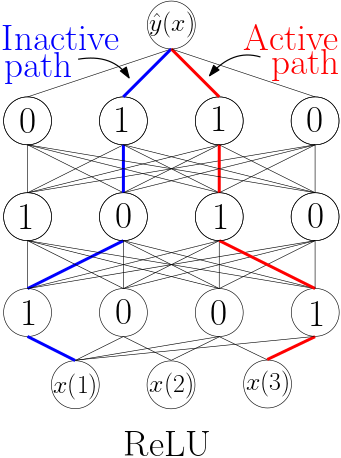
\includegraphics[scale=0.5]{figs/nn.png}
%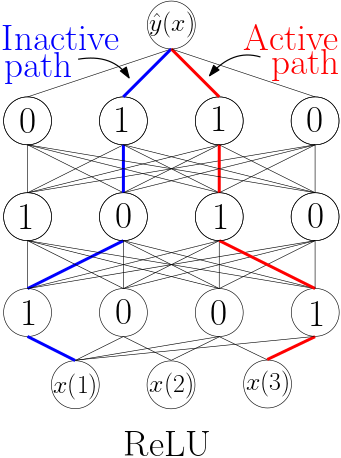
\includegraphics[scale=0.5]{figs/nn.png}
\end{tabular}
}
%\end{minipage}
%\begin{minipage}{0.18\columnwidth}
%\resizebox{\columnwidth}{!}{
%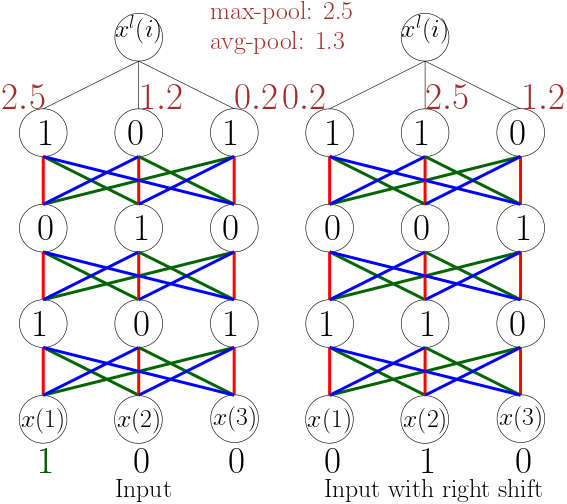
\includegraphics[scale=0.5]{figs/nnconv.png}
%}
%\end{minipage}
\caption{Activations and Gates}
\label{fig:actgate}
\end{figure*}
\begin{table}[h]
\centering
\resizebox{\columnwidth}{!}{
\begin{tabular}{|c|c|c|c|}\hline
		&Gate&Activation&$\dot{\chi}$\\\hline
Prior&$G_r(q)=\mathbbm{1}_{\{q>0\}}$& $\begin{aligned}\chi_{r}(q)&=q\cdot\mathbbm{1}_{\{q>0\}}\\ \chi_{sp}(q)&=\frac{1}{\beta}\log(1+\exp(\beta q))\end{aligned}$&$\begin{aligned}\dot{\chi_{r}}(q)&: \text{Heaviside step function} \\ \dot{\chi}_{sp}(q)&=\frac{1}{1+\exp(-\beta q)}\end{aligned}$ \\\hline
Ours &$G_{sr}(q)=\frac{1}{1+\exp(-\beta q)}$ &$\chi_{sr}(q)=q\cdot G_{sr}(q)$& $\dot{\chi}_{sr}(q)=\dot{\chi}_{sr}(q)+\underbrace{\dot{G}_{sr}(q)}_{\text{Gate Dynamics}}$\\\hline
\end{tabular}
}
\caption{A comparison of prior work and our paper. Here `$sp$' stands softplus.}
\label{tb:compare}
\end{table}

The soft-ReLU activation plays a key part: note that, in prior works, in the expression for the limit NTK $K^{(d)}$ in \eqref{eq:ntkold}, $\dot{\chi}$ is either a Heaviside step function or a logit function. Both these functions capture the \emph{on/off} behaviour of the gates, and hence the $K^{(d)}$ captures only the flow of value gradient through the active sub-networks. On the contrary, in the case of soft-ReLU (see row $3$ of \Cref{tb:compare}), $\dot{\chi}_{sr}$ contains both the \emph{on/off} information via the $\dot{\chi}_{sp}$ term as well as the information on the dynamics of sensitive gates via the $\dot{G}_{sr}$ term.

Plugging the soft-ReLU instead of softplus/ReLU in \eqref{eq:ntkold} will indeed bring in the additional terms related to gate dynamics (see last row of \Cref{tb:compare}) in $K^{(d)}$. However, note that $K^{(d)}$ is a single matrix, and only due to the `path-view', we can identify its components namely $K^v_{\Theta}$, and $K^{\phi}_{\Theta}$ which have completely different functions.
\subsection{Gradient Dynamics in `Large-Width' Regime }
\end{comment}
% $K^v_{\Theta}$ in \eqref{eq:graddyna} converges to $K^{(d)}$ in \eqref{eq:ntkold} with $\chi=\chi_{sr}$, and $\dot{\chi}=\dot{\chi}_{sp}$ (since $\dot{\chi}_{sr}=\dot{\chi}_{sp}+\dot{G}_{sr}$ and in $K^v_{\Theta}$, $\dot{G}_{sr}$ term is $0$).\\